% !TeX spellcheck = en_US
\chapter{Methodology}%
\section{Internal}
\subsection{Overview (conceptual diagram)}



%figure conceptual MAS
\begin{figure}[htb]
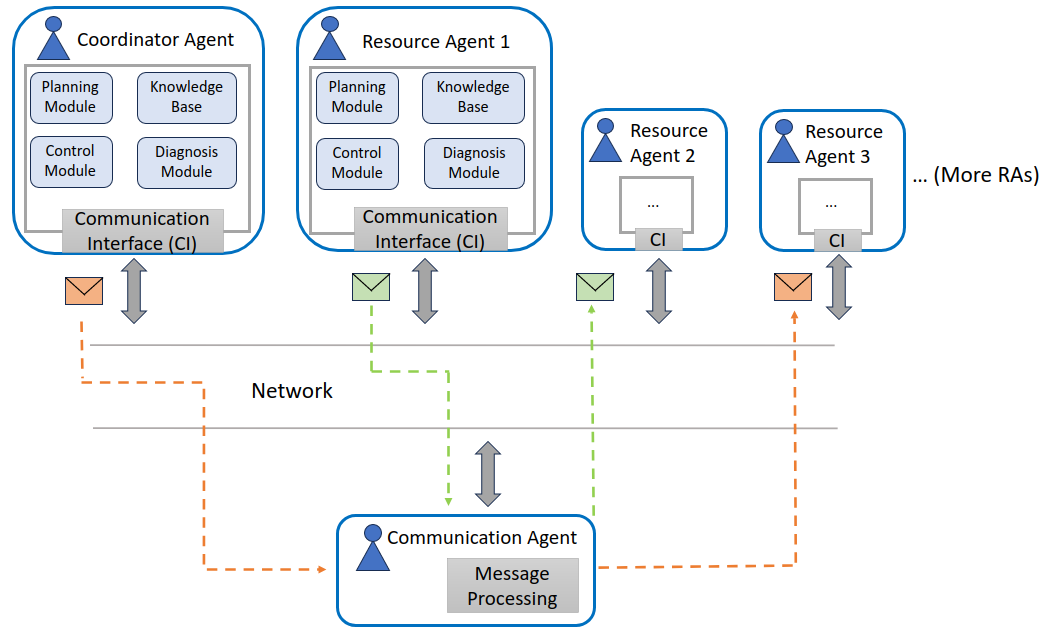
\includegraphics[width=16cm]{figures/MAS_Conceptual_Diagram.png}
\centering
\caption{Conceptual diagram of MAS\label{fig: MASConceptual}}
\end{figure}

% decribe the conceptual diagram

In the Figure.\ref{fig: MASConceptual} shows a conceptual diagram of a \gls{mas} based on the \gls{ra} design patterns in Wannagat’s architecture, with the focus on communication between agents, planning and decision making inside each agent. The \gls{cda} here is identical to \gls{ams} of Wanagat, which should also be counted as an agent instead of a management system. The five modules within an agent are: 
\begin{itemize}
\item Planning Module
\item Control Module
\item Knowledge Base
\item Diagnosis Module
\item Communication Interface.
\end{itemize}

Each module within a Coordinator agent or a \gls{ra}
Based on these five modules, the task to be executed in an agent should also be categorized into 5 parts. The following table shows some tasks of each module based on the general requirements of a smart factory.



\begin{table}[]
\caption{Wanagat's \gls{ra} design patterns with task related examples.}
\label{tab:designPatterns}
\renewcommand{\arraystretch}{1} 
\setlength{\extrarowheight}{3pt}

\begin{tabular}{|m{2cm}|m{4cm}|m{8cm}|}
\hline
\multicolumn{3}{|c|}{ Wanagat's design patterns} \\ % Header with background color
\hline
Module name& Task &Example \\ 
\hline
\begin{tabular}[c]{@{}p{2cm}@{}} Planning Module \end{tabular} & \begin{tabular}[c]{@{}p{4cm}@{}} \textbullet\  Task planning \\ \textbullet\ Decision making \\ \textbullet\ Resource allocation \\ \textbullet\ Sequencing \\ \textbullet\ Scheduling\end{tabular} 
& \begin{tabular}[c]{@{}p{8cm}@{}} \textbullet\ Break down tasks into smaller executable units\\ \textbullet\ Decide which task should be assigned to which agent \\ \textbullet\ Allocate the agents with specific tasks \\ \textbullet\ Find the task execution sequence \\ \textbullet\ Calculate the execution time for each agent\end{tabular}  \\ 
\hline

\begin{tabular}[c]{@{}p{2cm}@{}} Control Module \end{tabular}& \begin{tabular}[c]{@{}p{4cm}@{}} \textbullet\ Monitoring \\ \textbullet\ Adaptation \\ \textbullet\ Control and optimization \\ \textbullet\ Resource allocation \\ \textbullet\ Actuation\end{tabular} 
& \begin{tabular}[c]{@{}p{8cm}@{}} \textbullet\ Acquisition of robot states\\ \textbullet\ Adapt the plans with
current state, e.g.: emergent stop \\ \textbullet\ Control and optimize the robot’s motion \\ \textbullet\ Allocate the agents with specific tasks \\ \textbullet\ Actuate the robot with outputs\end{tabular}  \\ 
\hline

\begin{tabular}[c]{@{}p{2cm}@{}}Knowledge Base \end{tabular} & \begin{tabular}[c]{@{}p{4cm}@{}} \textbullet\ \gls{db} \\ \textbullet\ Knowledge representation and reasoning \\ \textbullet\ Learning \\ \textbullet\ Knowledge sharing\end{tabular} 
& \begin{tabular}[c]{@{}p{8cm}@{}} \textbullet\ Hierarchical, relational, non-relational and object oriented\\ \textbullet\ Relational ontology \gls{db} system \\ \textbullet\ Agent learns from the existing primitives
and create new executable primitives for customer’s changing
requirements \\ \textbullet\ Unfound primitives
could be retrieved by querying other agents\end{tabular}  \\ 
\hline

\begin{tabular}[c]{@{}p{2cm}@{}} Diagnosis Module \end{tabular} & \begin{tabular}[c]{@{}p{4cm}@{}} \textbullet\ Fault detection \\ \textbullet\ Fault diagnosis \\ \textbullet\ Root cause analysis and classification \\ \textbullet\ Fault prediction\end{tabular} 
& \begin{tabular}[c]{@{}p{8cm}@{}} \textbullet\ Monitor the time-series data to detect anomalies from robot states, e.g.: detect faulty joint values for abortion\\ \textbullet\ More complex analysis to diagnose faulty patterns with mathematical algorithms and models, or AI-based methods \\ \textbullet\ Find the reasons for anomalies and categorize them for patterns recognition \\ \textbullet\ predict the system faults by learning the classification models\end{tabular}  \\ 
\hline

\begin{tabular}[c]{@{}p{2cm}@{}} Communi-cation Interface \end{tabular}& \begin{tabular}[c]{@{}p{4cm}@{}} \textbullet\ Message parsing and encoding \\ \textbullet\ Connection establishment and maintenance \\ \textbullet\ Message handling \\ \textbullet\ Data security\end{tabular} 
& \begin{tabular}[c]{@{}p{8cm}@{}} \textbullet\ Encode and decode the messages in agent specific data type, or parse the data object to other types, e.g.: json\\ \textbullet\ Ensure the connection with other agents based on system requirements \\ \textbullet\ Filter messages with undesired data type or incomplete messages, and prioritize the incoming messages \\ \textbullet\ Ensure data integrity and confidentiality, by encrypting, decrypting and authenticating messages to avoid cyber attack\end{tabular}  \\ 
\hline

\end{tabular}

\label{tab: designPatternsTable}
\end{table}







\subsection{Prerequisite}
\subsubsection{System Setup}
 
%figure conceptual MAS
\begin{figure}[htbp]
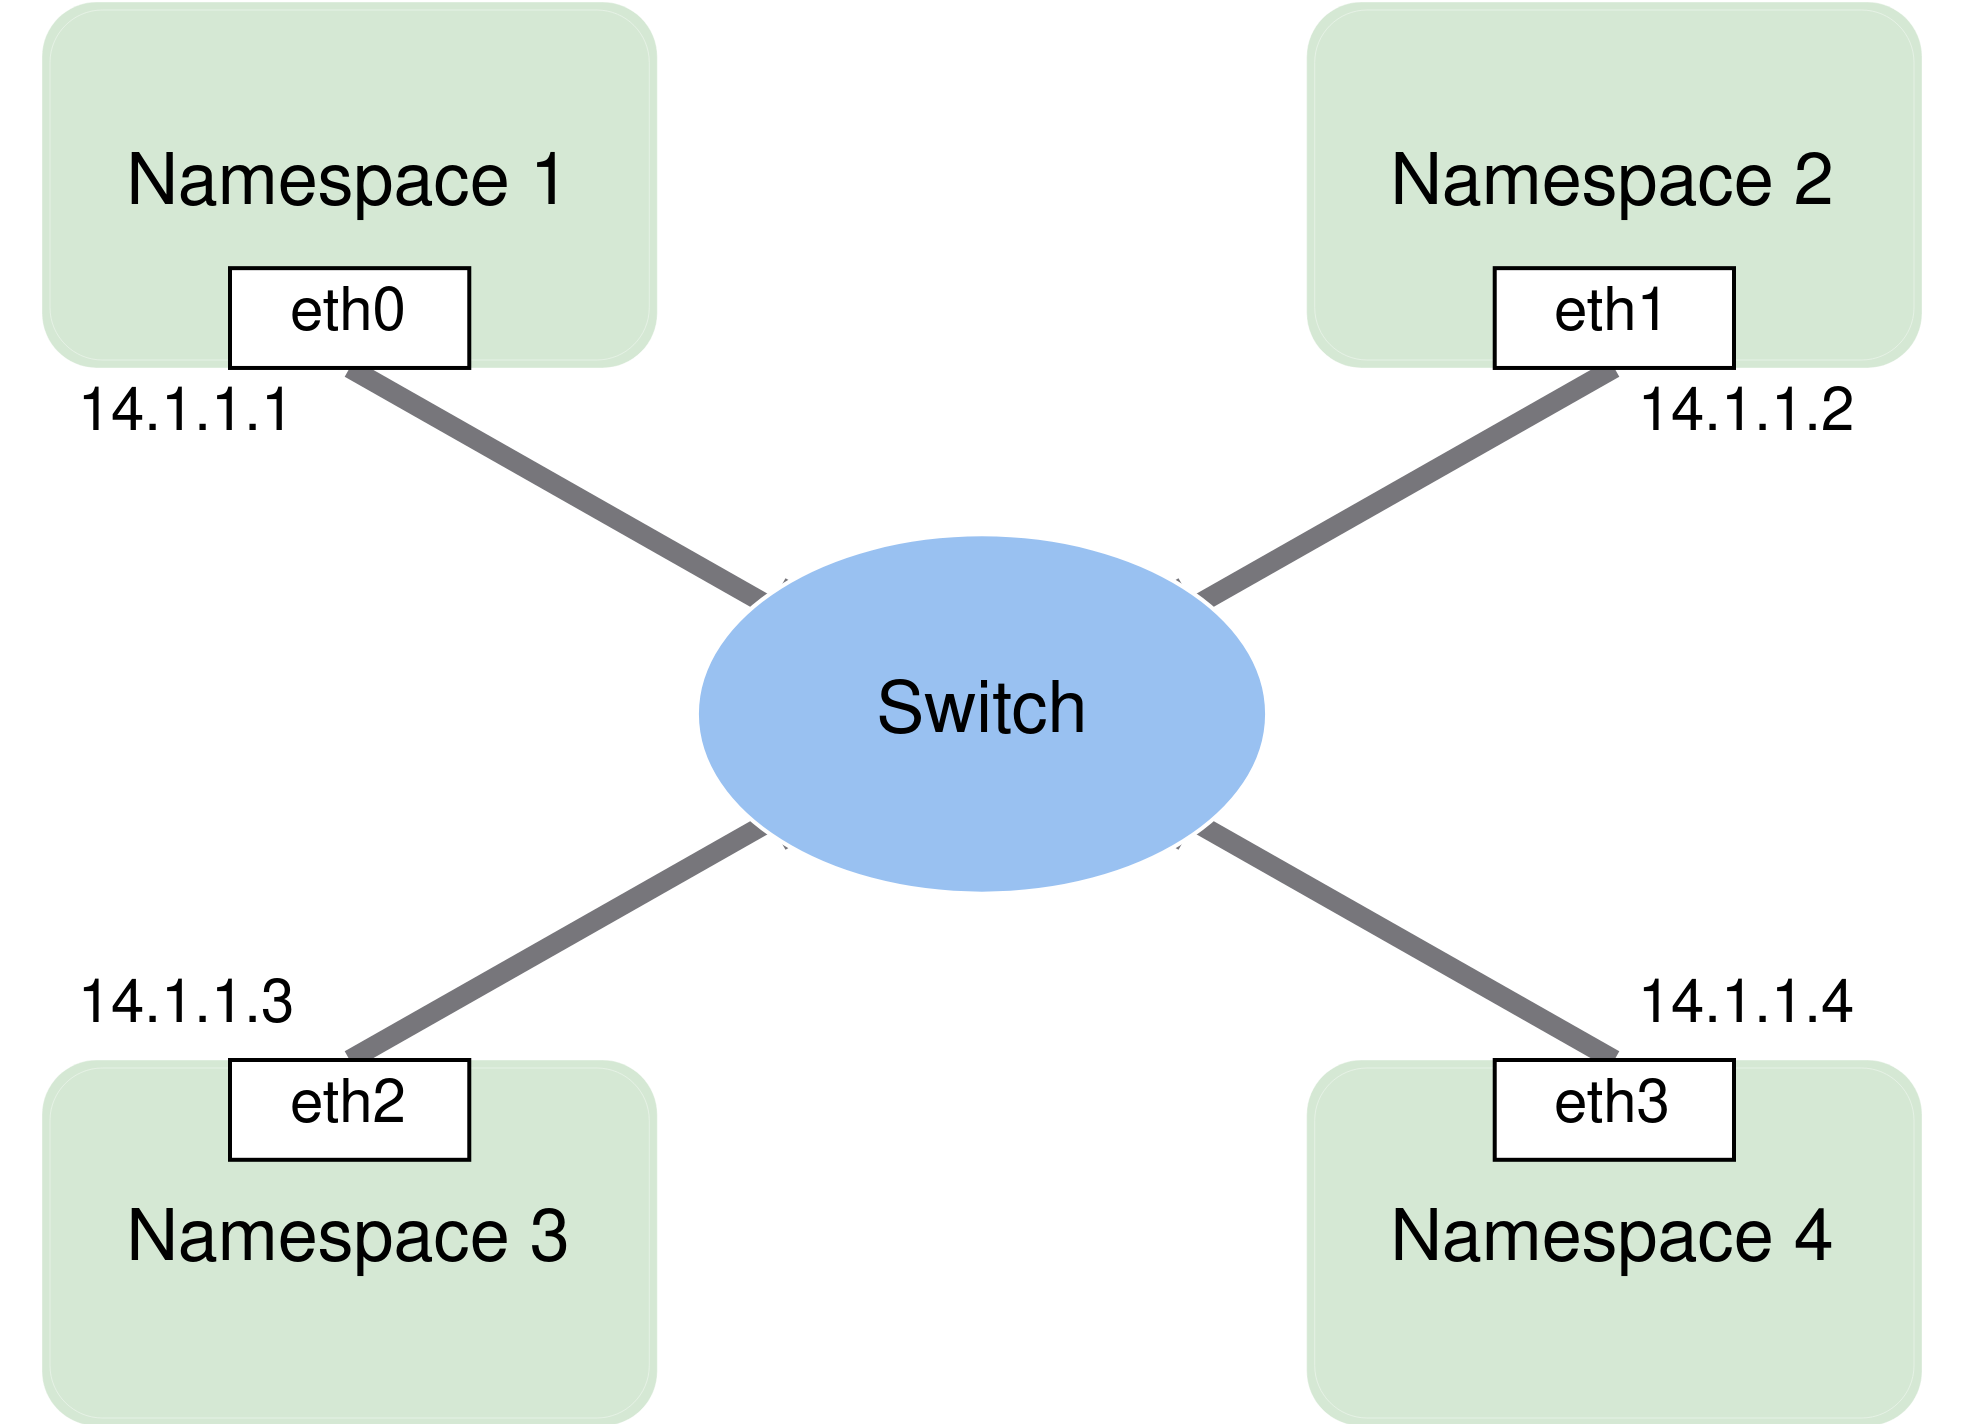
\includegraphics[width=12cm]{figures/NamespaceConceptual.png}
\centering
\caption{Conceptual diagram of namespaces creation
\label{fig: NSConceptual}}
\end{figure}

In order to emulate network environments for agent's communication testing and development of the \gls{mas}, the internal packets routing between agents in a single Linux device should be avoided. A common way to visualize the network to do performance testing is to use namespaces for network emulation. The trick is that a process running within a given namespace will see only the network interfaces, including virtual interfaces, forwarding tables, etc., that exist in that namespace. The applications under test should serve as a switch and each packet should be routed through these interfaces. The Figure.\ref{fig: NSConceptual} shows that, each namespace is assigned with a virtual ethernet interface, starting with the name eth, which is configured with an individual IP address. Each time a script gets called, it is running under a namespace with its own IP address. In exercise, if a packet is sent from Namespace 1 to Namespace 3 and then back, it is routed by the switch intead of bridges between namespaces, which are not configured here in order to avoid internal routing.

\subsection{OSI model and comparison between sockets relevant protocol layers}
%figure conceptual MAS
\begin{figure}[htbp]
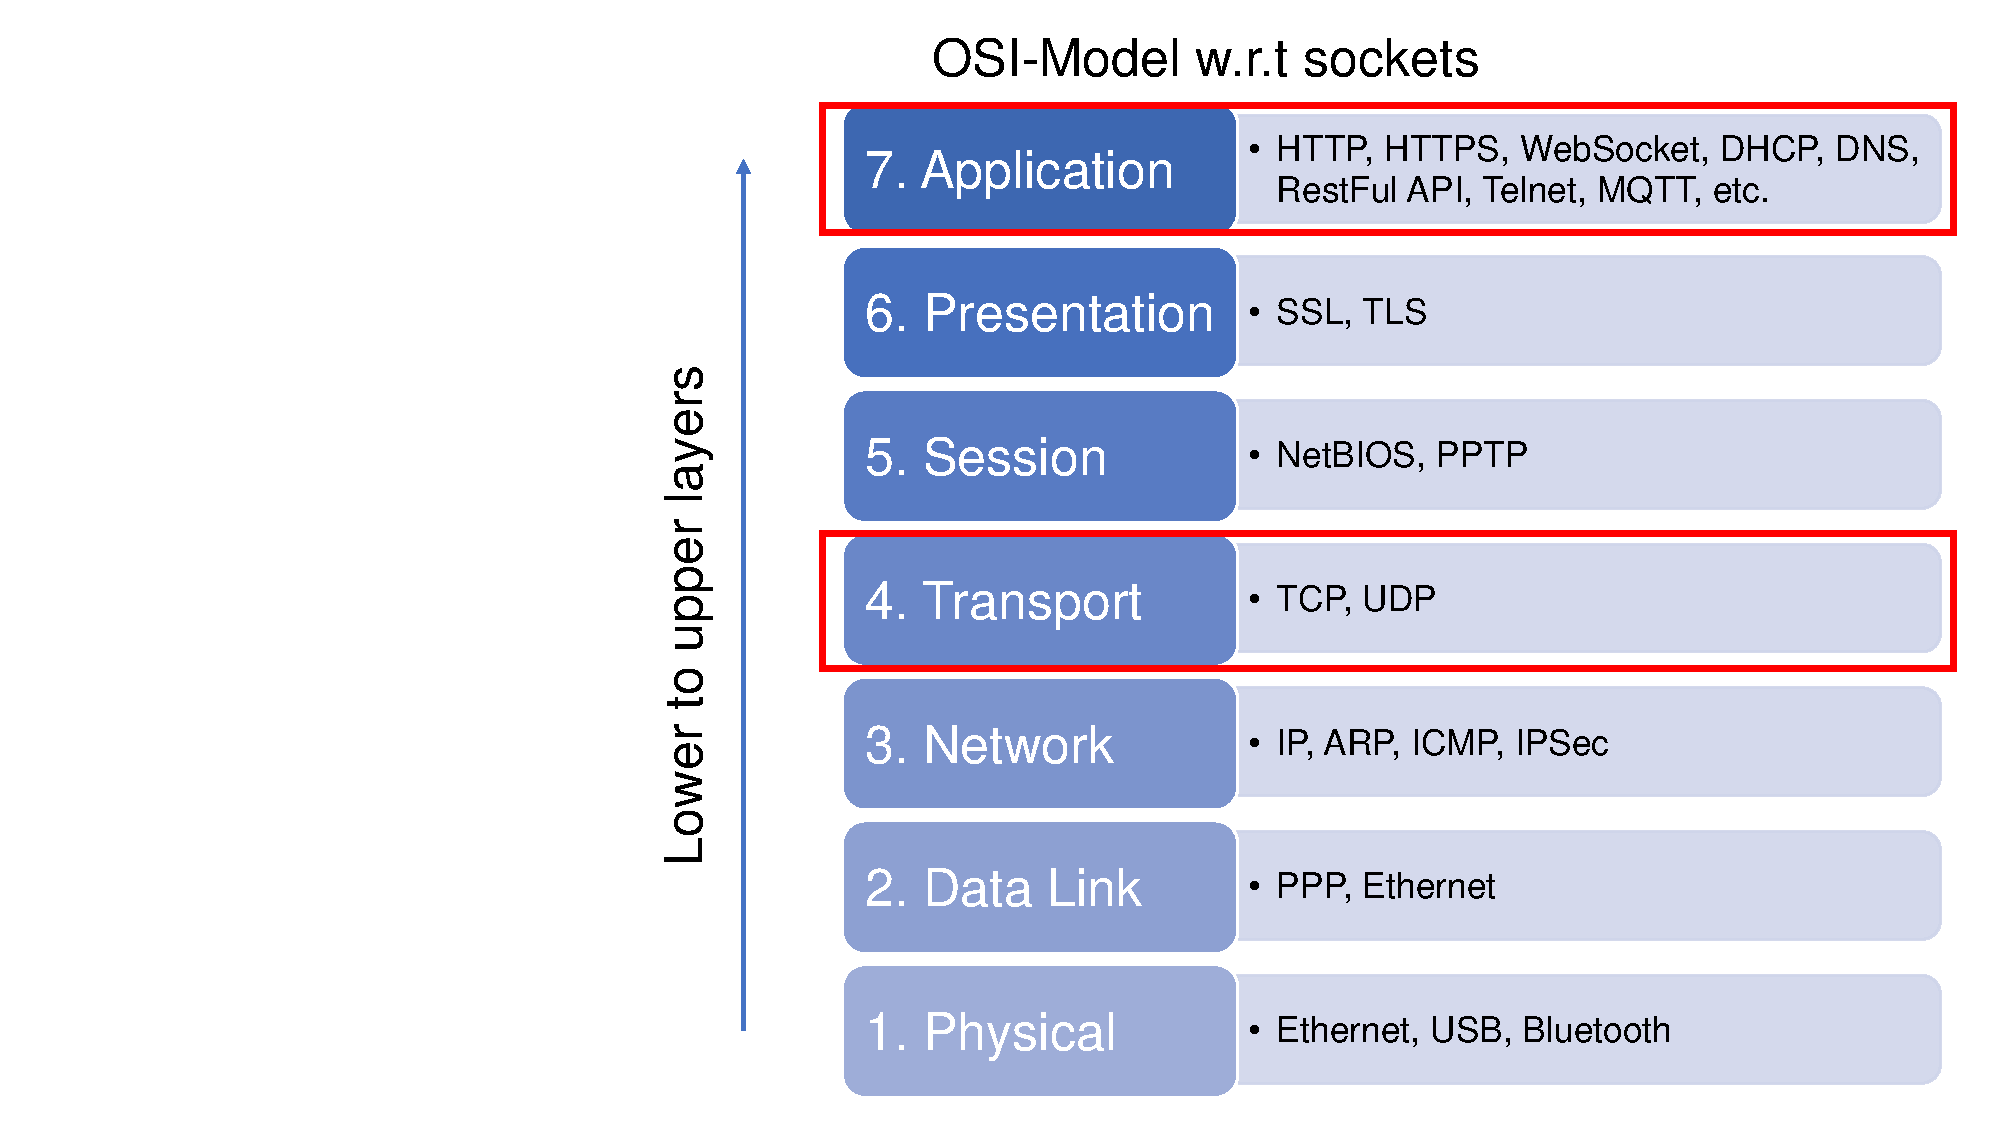
\includegraphics[width=12cm]{figures/OSI.pdf}
\centering
\caption{Conceptual diagram of Namespaces creation\label{fig: OSI}}
\end{figure}

Figure. \ref{fig: OSI} shows the famous OSI-Model with 7 abstraction layers with Transport layer and application layers most relevant to sockets. TCP and UDP are typical transport layer protocols and they provide an end-to-end data transport between two devices while the application layer protocols like HTTP or Websocket establish a communication between applications within devices. Although the application layer protocols still utilize TCP/UDP sockets to transport stream data, they defined additional "rules" to specify structure, content, and semantics of the messages transport through sockets. In the following tables, a comparison between sockets in different layers provide a more straight forward overview of their pro and cons in different contents.

% Please add the following required packages to your document preamble:
% \usepackage{graphicx}
% \usepackage{tabularx}

\begin{table}[htbp]
\small
\centering
\caption{Characteristics of different technologies in transportlayer protocols}
\label{tab: transportlayer}
\begin{tabular}{|m{0.2\textwidth}|m{0.3\textwidth}|m{0.3\textwidth}|}
\hline
\multicolumn{3}{|c|}{\textbf{Transport layer protocols}}                                                            \\ \hline
\textbf{Aspect}                         & \textbf{\gls{tcp}}             & \textbf{\gls{udp}}        \\ \hline
Use cases                      & Web browsing, email, text messaging, and file transfers & Live and real-time data transmission \\ \hline
Reliability                    & Reliable        & Unreliable \\ \hline
Stream type                    & Byte stream with no preserved boundaries & Message stream with preserved boundaries \\ \hline
Connection type                & Connection oriented, three handshake & No connection needed \\ \hline
Overhead                       & Larger than \gls{udp} & Very low   \\ \hline
Header size                    & 20-60 bytes     & 8 bytes    \\ \hline
Sequence                       & Packets arrive in sequence & No sequencing for packets \\ \hline
Retransmission of lost packets & Yes             & No         \\ \hline
Speed                          & Slower than \gls{udp}, because of overhead and connection & Relative faster than \gls{tcp} \\ \hline
State                          & Stateful        & Stateless  \\ \hline
Flow control                   & Yes             & No         \\ \hline
\end{tabular}
\end{table}




% % Please add the following required packages to your document preamble:

\begin{sidewaystable}[htbp]
\small
\caption{Characteristics of different technologies in application layer protocols}
\label{tab: applicationlayer}
\centering
\begin{tabular}{|m{0.13\textwidth}|m{0.2\textwidth}|m{0.2\textwidth}|m{0.2\textwidth}|m{0.2\textwidth}|}
\hline
\multicolumn{5}{|c|}{\textbf{Application layer protocols}} \\ \hline
\textbf{Aspect} & \textbf{HTTP} & \textbf{WebSocket} & \textbf{RESTful API} & \textbf{MQTT} \\ \hline
Use cases & Web pages, images, videos, World Wide Web, etc & Such as chat applications, live gaming, etc & Web and mobile applications with data management requirement & Usually in IoT with limited bandwidth \\ \hline
Functionality & Request-response protocol based on TCP, foundation for both RESTful APIs and the initial connection in WebSockets & Bi-directional, real-time communication & Uses standard HTTP methods to perform CRUD (Create, Read, Update, Delete) & Lightweight message transport, runs over TCP \\ \hline
Security & Use SSL/TLS & ws (unsecured) and wss (secured with SSL/TLS) & Similar to HTTP, can be further secured using various authentication mechanisms like OAuth, JWT & Use TLS, like username/password authentication and optional message-level security \\ \hline
Message patterns & Request-Response & Full Duplex (send and receive independent) & Request-Response & Publish-Subscribe \\ \hline
Connection type & No connection needed & Persistent {connection} & No connection needed & Persistent connection \\ \hline
State & Stateless & Stateful & Stateless & Stateful \\ \hline
Overhead & Overhead for each request-response cycle, especially for new connections & After the initial handshake (HTTP), data frames are lightweight & Similar to HTTP, dependent on API design & Minimal message overhead \\ \hline
Realtime capability & Less Capable & Highly Suitable & Variable & Highly Suitable \\ \hline
Flexibility & Supported in all environments & Supported in most modern web browsers and many backend environments & Similar to HTTP & Highly flexible \\ \hline
Adaptability to dynamic changes & Relative lower (influenced by stateless nature) & High & Relative lower (influenced by stateless nature) & High \\ \hline
Capability of handling instability & Less capable, requires a stable connection for each request-response cycle & Less stable if connection disruptions happen frequently & Identical to HTTP & Capable, Ideal for remote locations with limited connectivity \\ \hline
Scalability & Less scalable, require more infrastructure support & Highly scalable, maintains connections for real-time interactions & similar to HTTP, dependent on API design & Highly scalable based on broker-client message transport \\ \hline
\end{tabular}
\end{sidewaystable}


Table \ref{tab: transportlayer} compares the typical transport layer protocols \gls{tcp} and \gls{udp} from different aspects.  \gls{tcp} provides reliable data transfer while \gls{udp} mainly focuses on transport speed and efficiency without reliability guarantee. With the focus on speed and reliability, \gls{udp} on one hand offers a faster packet transfer, while on the other hand produces a network dependent packet loss rate and out-of-order packet sequence, compared to \gls{tcp}. Because of the requirement of a reliable real time ordered data transfer with minimum to no packet loss in \gls{mas} communication, TCP is used as the base protocols of the design. There are several protocols in application layers that are considered to be suitable for \gls{mas} communication, each with its own advantages and limits in different aspects according to table \ref{tab: applicationlayer}.
To get a closer look of the Table \ref{tab: applicationlayer},  a horizontal comparisons between different application layer protocols: 
\begin{itemize}
\item \gls{http},
\item WebSocket,
\item RESTful API,
\item and \gls{mqtt},
\end{itemize}
should be performed. In one word, WebSocket is chosen to be the application layer protocols for MAS communication, while \gls{tcp} socket for the \gls{dt} agent design, which will be further discussed in the next chapter. Here are the reasons of the choice of WebSocket: 
\begin{enumerate}
\item Bi-directional, full duplex, real time communication between server and clients, no re-connection needed. Suitable for continuous data transfer.
\item Overhead small after connection establishment to reduce latency(\gls{http}).
\item Stateful, store the information of the client's state under connection.
\item High flexibility, adaptability and scalability
\item Secure with wss.
\end{enumerate}

Figure.\ref{fig: MsgConceptual} shows the differences between bi-directional full duplex and other message patterns like Request-Response and Publish-Subscribe, in the context of data transfer. For the \gls{mqtt}, publisher publish (send) a message within a topic to the broker (server), while subscriber subscribes (receive) the message from the broker within the same topic. For response, a new topic needed to be started, but there is no guarantee that the original publisher is listening, which is a drawback for send-and-receive patterns of \gls{mas}. 

Relatively, the other three protocols will be considered as more appropriate. For instance both HTTP and RESTful API run in request-response mechanism. A client posts (sends) messages to the server for the other client will get (receive) from it. Whether the GET and POST method are successful or not, a response will be given back. With this mechanism, each time a message is going through the server, a new connection will be established and closed after responses are sent. The inconsistent connection will consume more communication time and lead to higher latency. The ideal solution for that is the bi-directional and full duplex real time communication mechanism of WebSocket. Basically the client sends a message to the server, after processing the data, the server will pass the message to the other client and receive response with the same logic. This allows simultaneous communication in both directions between clients, so that no re-connection in the message transfer cycle is necessary. The consistent server-client connection makes it possible to realize a continuous real time communication between agents. In the next section, a more detailed explanation of WebSocket mechanism will be given.

%figure conceptual application layer protocols
\begin{figure}[htb]
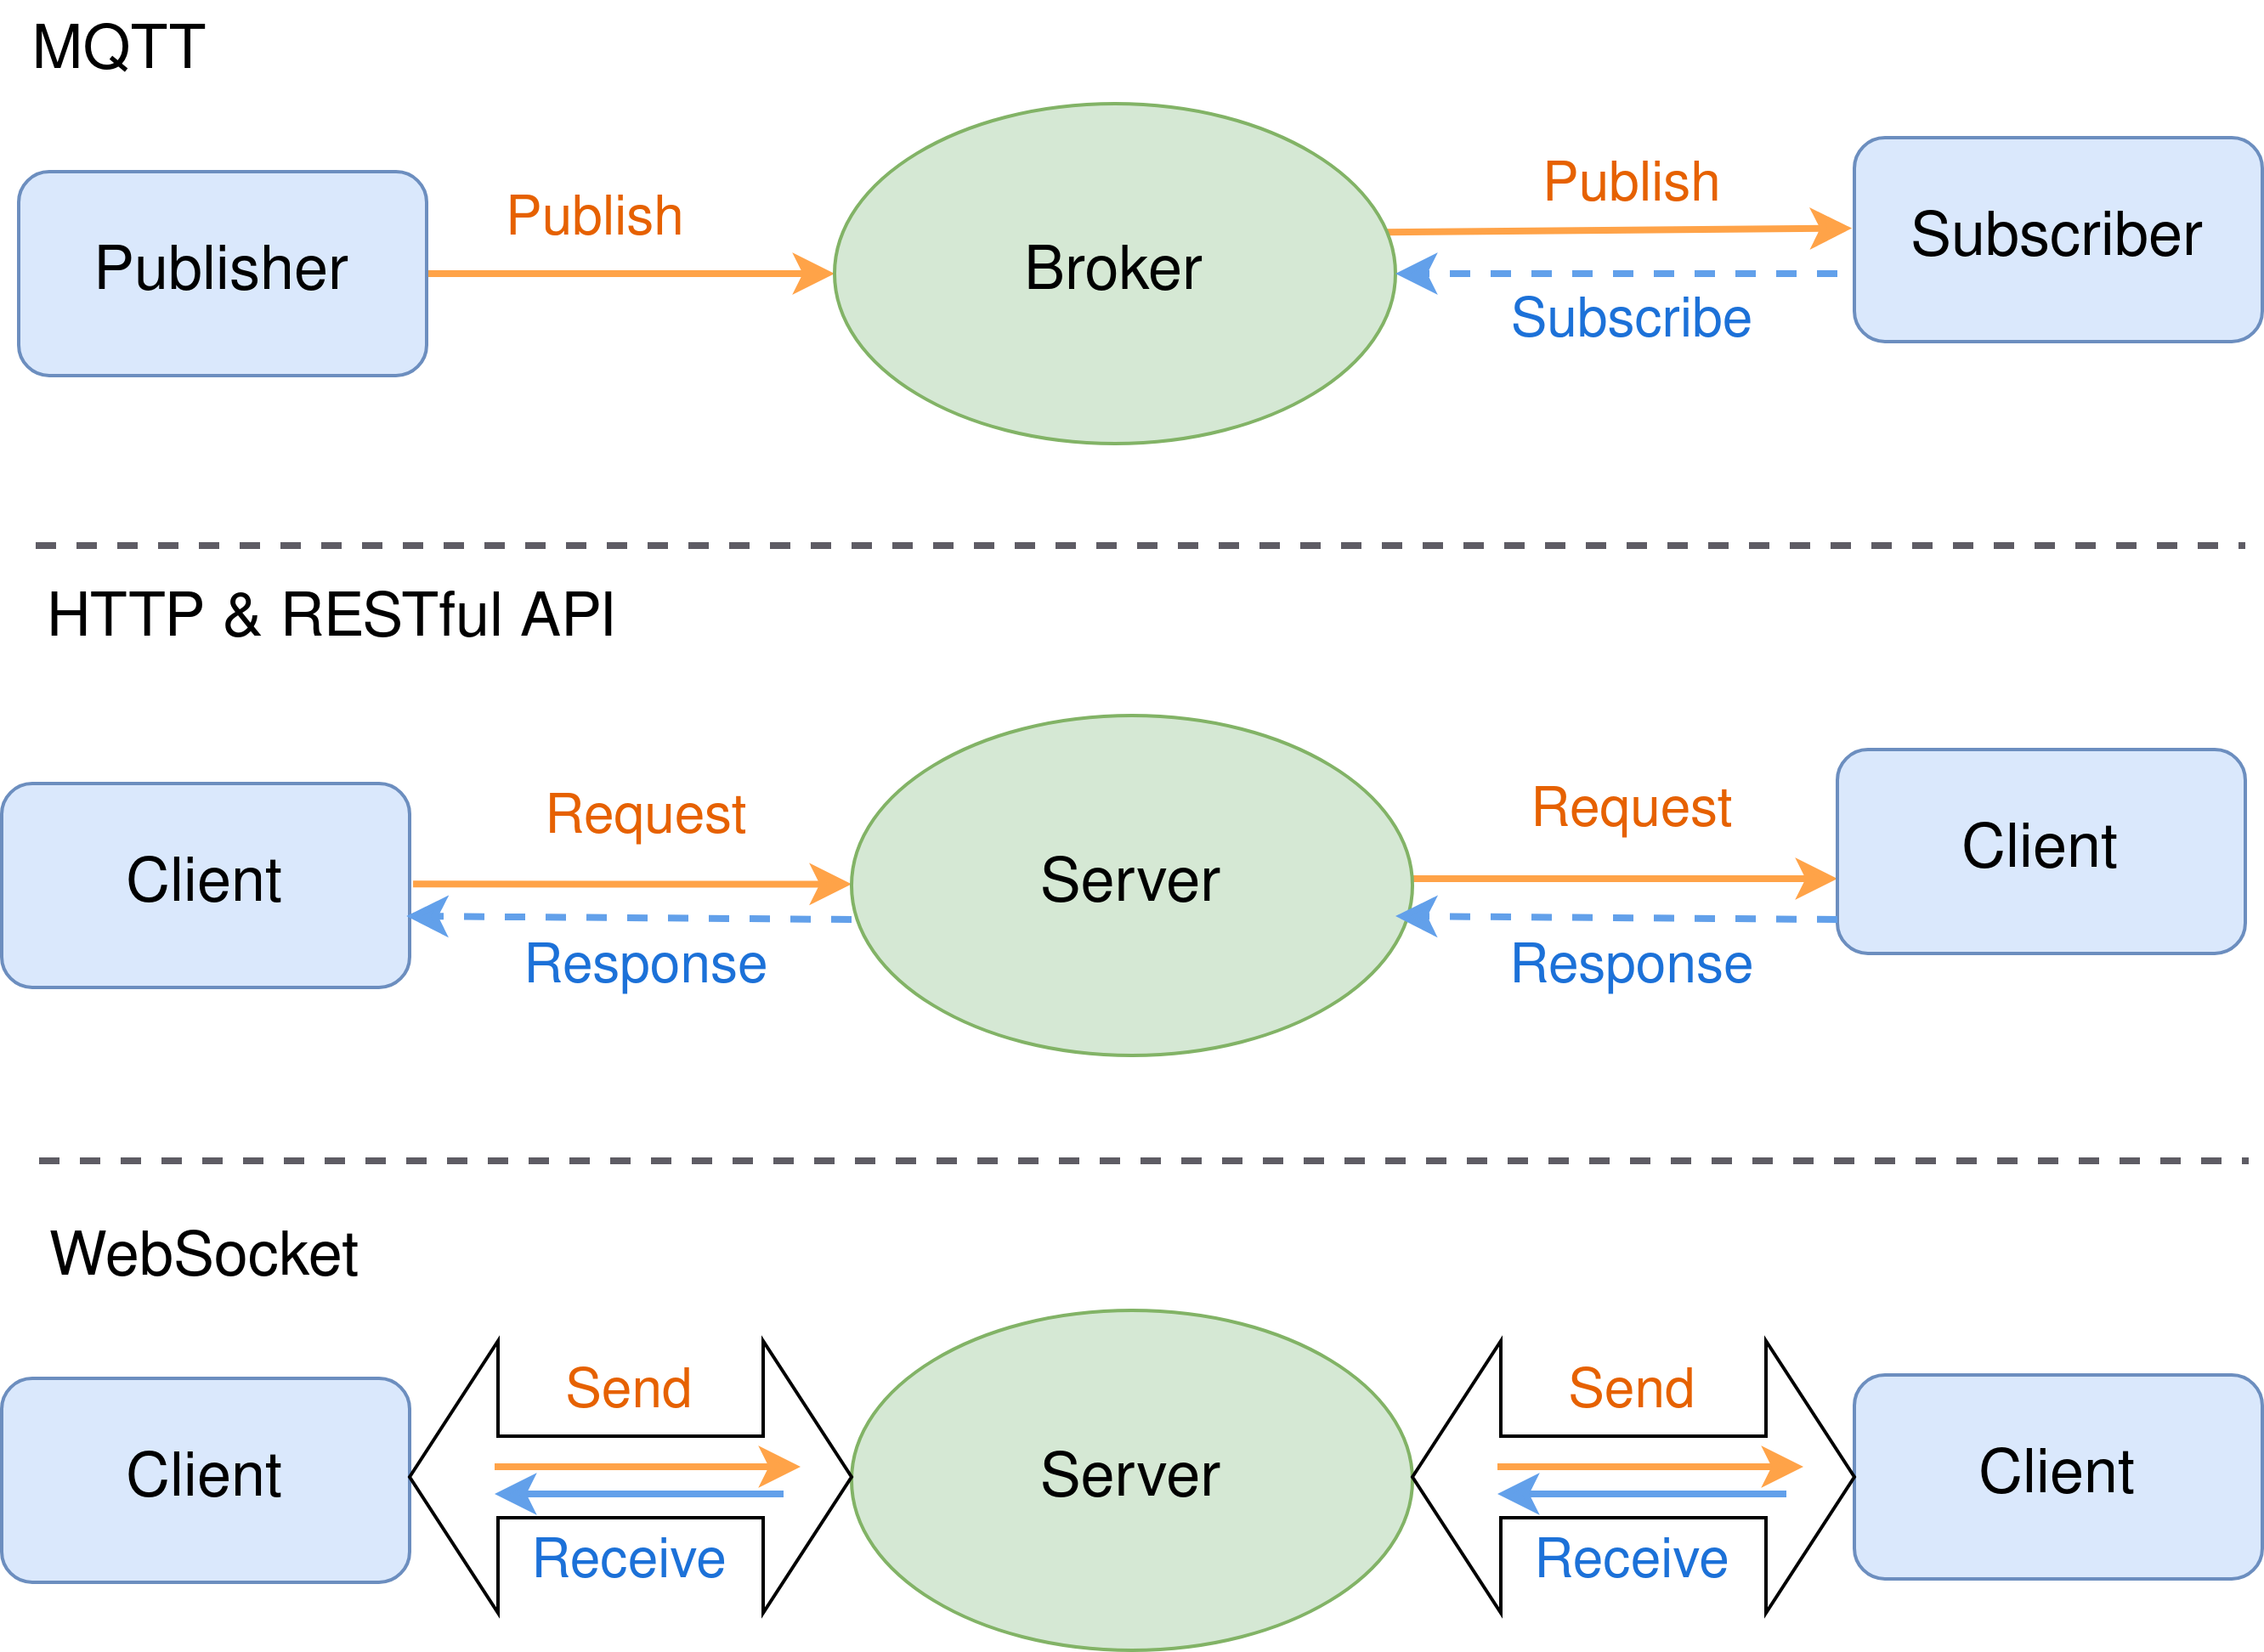
\includegraphics[width=12cm]{figures/MessageConceptual.png}
\centering
\caption{Conceptual diagram of MAS\label{fig: MsgConceptual}}
\end{figure}




\subsection{Pseudo-Code of MAS workflow}
% Define Class...EndClass for better representation
\algnewcommand\algorithmicclass{\textbf{class}}
\algdef{SE}[CLASS]{Class}{EndClass}[1]
   {\algorithmicclass\ \textsc{#1}\vspace{0.2cm}}%
   {\vspace{0.2cm}}%
   
\begin{algorithm}
\caption{Pseudo-Code of Coordinator agent in MAS workflow}
\label{alg:CDAPseudoCode}
\begin{algorithmic}
\State \textbf{Import} necessary libraries
\State \textbf{Initialize} agent relevant variables

\State \textbf{Class} messageSender
    \Procedure{send\_and\_receive\_messages}{$self, recipient, message, priority$}
    \State 1. Establish a WebSocket connection
    \State 2. Send and receive messages
    \State 3. Handle exceptions
    \EndProcedure
\State \textbf{EndClass}
\State \textbf{Class} messageReceiver
    \Procedure{receive\_and\_send\_messages}{$self, recipient, message, priority$}
    \State 1. Establish a WebSocket connection
    \State 2. Receive and send messages
    \State 3. Handle exceptions
    \EndProcedure
\State \textbf{EndClass}
\State \textbf{Class} agentsAllocation
    \Procedure{allocate\_agents\_with\_sequenced\_primitives}{$self, requirements$}
    \State 1. Find tasks from customer requirements
    \State 2. Breakdown tasks into skills
    \State 3. Breakdown skills into primitives
    \State 3. Allocate agents
    \EndProcedure
\State \textbf{EndClass}

\State \textbf{Main:}
\State \textbf{Instantiate} allocated agents and message sender and receiver
\State \textbf{Loop} for each agent to check connection
\State \textbf{Loop} for each agent to check capabilities
\State \textbf{Notify} agents about finished checks
\State \textbf{Loop} to send sequence and agent information
\State \textbf{Start} availability checks
\State \textbf{Loop} to receive and send messages
\end{algorithmic}
\end{algorithm}

\subsection{tcp socket and websocket}
compare tcp and websockets in programming difference (server, clients)


\section{External}
\subsection{Overview (conceptual diagram)}

%figure conceptual DT
\begin{figure}[htb]
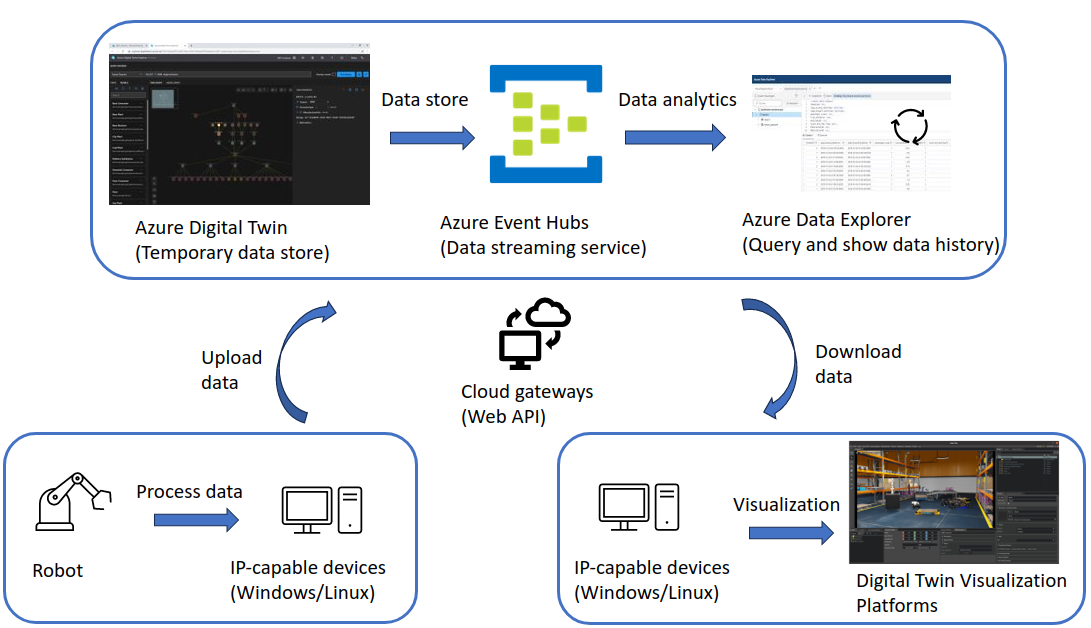
\includegraphics[width=16cm]{figures/DT_Conceptual_Diagram.png}
\centering
\caption{Conceptual diagram of MAS\label{fig: DTConceptual}}
\end{figure}



\subsection{Prerequisite}
System Setup: 


1. NTP setup


2. packages installation for tcp sockets


\subsection{Pseudo-Code}
Pseudo-Code of workflow of RCP-DTAgent

\subsection{MS Azure Digital Twin}
Azure Digital twin database setup